%% Generated by md2ieee.py from R4_draft.md -- edit the Markdown, then regenerate.
\documentclass[conference]{IEEEtran}
\usepackage{cite}
\usepackage{graphicx}
\graphicspath{{../figures/}{figures/}{./}}
\usepackage{booktabs}
\usepackage{tabularx}
\usepackage{amssymb}
\usepackage[hidelinks]{hyperref}
\newcommand{\inferred}{\textsuperscript{\dag}}
\newcommand{\artifact}[1]{{\footnotesize [artifact: #1]}}
\begin{document}
\title{What Would a Black-Box Tester Need? Real Access-Control Vulnerabilities in OpenAPI-Described REST Services}
\author{\IEEEauthorblockN{Anonymous Author(s)}\IEEEauthorblockA{Under double-anonymous review}}
\maketitle
\begin{abstract}
Black-box REST API testers increasingly hunt for broken access control: they take an OpenAPI document and a few credentials and judge responses with oracles, yet their positive findings of missed authorization checks come mostly from seeded or example services. We ask what such a tester would need to expose \emph{real} access-control vulnerabilities, and whether the contract carries the information an oracle needs. From 2,025 reviewed GitHub security advisories with access-control weaknesses in the Maven and Go ecosystems, we froze a pool of 176 fixed vulnerabilities in services that ship an OpenAPI document and sampled 138 from 70 repositories; two GPT-family and two Claude-family coders classified each advisory and fix blind, under a pre-registered, hash-frozen protocol. 102 (74\%) are access-control flaws reachable over HTTP. Of the 89 with a decided setup, only about half (49, 55\%) need two principals to expose: object-level and tenant-isolation flaws mostly need two users of the same role and function-level flaws mostly two roles, while all missing-authentication flaws yield to an anonymous request and most property-level flaws to a single user (40 of 89); 13 remain undecided. Almost all violations (101/102) are observable in HTTP responses, but the contract rarely helps: the vulnerable operation is clearly described in only 41 cases, and when it is, the violated rule is absent in 33 of 38 (87\%; p = $2.1 \times 10^{-6}$); fixes leave the contract untouched in 93 of 102 (91\%). The two model families agree on vulnerability kind ($\kappa$ 0.83). Contract-driven oracles must infer access rules rather than read them, and testers need multi-principal setups for about half of real cases.
\end{abstract}

\section{Introduction}
Broken access control is the most critical class of API vulnerability: object-level authorization ranks first in the OWASP API Security Top 10. Automated REST testers mostly work black-box:
\begin{itemize}
\item Schemathesis, RESTler and EvoMaster take an OpenAPI document and credentials, generate requests, and judge responses with oracles.
\item Recent tools add access-policy oracles that compare the responses of different users.
\end{itemize}

Their evaluations combine seeded faults, vulnerable-by-design services and real APIs, but positive findings for missed authorization checks come from the former. For example, Arcuri et al. add three access-policy oracles to EvoMaster that need only the OpenAPI document and the logins of at least two users; their missed-check oracle found faults in a service with injected faults, but none in real APIs~\cite{arcuri2025access}. Recent fuzzing work names the core obstacle directly: broken access control ``is underexplored in automated testing due to key challenges: the lack of reliable oracles and the difficulty of generating semantically valid attack requests'' ~\cite{arXiv2507_15984}.

The usual answer to the oracle problem is the contract: the OpenAPI document says which operations exist and which security schemes protect them. But does the contract carry the information needed to recognise a real access-control violation? And what test setup would a black-box tester need to provoke one at all? We answer both questions on real, published, fixed vulnerabilities in open-source REST services that ship an OpenAPI document:

\begin{itemize}
\item \textbf{RQ1 (kinds).} Which kinds of access-control vulnerabilities occur?
\item \textbf{RQ2 (test setup).} What minimal black-box setup exposes them, by number and roles of principals, and is the violation observable through HTTP responses?
\item \textbf{RQ3 (contract information).} Does the contract describe the vulnerable operation, declare a security requirement for it, and state the violated rule?
\item \textbf{RQ4 (fix visibility).} Does the fix change the contract, and where in the code is it made?
\end{itemize}

\textbf{Contributions.}
\begin{enumerate}
\item A frozen, reproducible sample of real access-control advisories for Java, Kotlin and Go REST services, each linked to its fix commit and to the contract at the vulnerable version.
\item Measurements of the black-box setup these vulnerabilities require, and of the contract information available to detect them.
\item Evidence on whether such fixes are visible to contract consumers.
\item A pre-registered, two-model-family blind coding protocol and a replication package.
\end{enumerate}

\section{Background and Related Work}
\textbf{Black-box REST testing and security oracles.}
\begin{itemize}
\item Black-box testers generate requests from an OpenAPI document. Their default oracles detect crashes (5xx) and schema violations.
\item Access-policy oracles go further and compare responses across principals.
\item Evaluations use seeded faults, vulnerable-by-design services such as Juice Shop, and real APIs. On real APIs, the missed-check oracle of Arcuri et al. found no faults~\cite{arcuri2025access}.
\end{itemize}

\textbf{Real access-control vulnerabilities.}
\begin{itemize}
\item Huang et al. detect BOLA vulnerabilities in database-backed applications~\cite{huang2024bola}.
\item BACFuzz is a gray-box fuzzer for BOLA and BFLA in PHP web applications ~\cite{arXiv2507_15984}.
\item BOLAZ analyses the data flow of resource identifiers in RESTful APIs to prevent horizontal privilege escalation ~\cite{arXiv2507_02309}.
\item IDORacle mediates SQL sinks at runtime in Java ~\cite{arXiv2609_12426}.
\item A taxonomy of 107 HackerOne reports finds that 84 were confirmed BOLA, of which 11.9\% are vertical privilege failures ~\cite{arXiv2605_25865}.
\item BAC-Bench collects 46 real broken-access-control vulnerabilities from six web applications to benchmark LLM repair ~\cite{arXiv2610_34290}.
\end{itemize}

None of these works asks what a contract-driven black-box tester would need for real vulnerabilities, or whether the contract carries the violated rule.

\textbf{Contracts and silent change.} A companion study (under review; omitted for anonymity) sampled 136 commits that change behaviour-path code but no contract file, in 47 REST services. It found that 44\% of them change observable API behaviour, and that 91\% of the client-breaking ones touch no contract annotation. Here we ask the same question for security fixes.

\section{Study Design}
\emph{(Summarised from the frozen plan \texttt{plan/\allowbreak{}R4\_PLAN.md}.)}

\subsection{Advisories and fix commits}
We query the GitHub Advisory Database for reviewed advisories in the Maven and Go ecosystems with access-control-related CWEs: 284, 285, 639, 862, 863, 915, 269, 266, 425, 566, 708 and 306.

For each advisory, we take as the fix the first commit reference that resolves. References to the advisory's own source repository come first. The vulnerable version is the fix's first parent.

\subsection{Eligibility, pool and sample}
An advisory is eligible if all of the following hold:
\begin{itemize}
\item \textbf{Contract present.} At the vulnerable version, the repository has a checked-in file whose name contains \texttt{openapi} or \texttt{swagger}, with a \texttt{.yaml}, \texttt{.yml} or \texttt{.json} extension, outside test, example, mock and vendor paths.
\item \textbf{Source change.} The fix changes non-test Java, Kotlin or Go source.
\item \textbf{Size.} The fix has at most 2,000 changed source lines.
\end{itemize}

Advisories that share a fix commit are merged. The pool is hash-frozen before any package is built. We take all items, up to 160, with at most four per repository by a seeded draw.

\textbf{Resulting counts.}
\begin{itemize}
\item \textbf{Query.} It returned 2,025 advisories; 53 were withdrawn.
\item \textbf{Fix commits.} 945 advisories cite no fix commit, and one commit could not be fetched. 1,026 resolved to a fix commit.
\item \textbf{Pool.}
\begin{itemize}
\item 831 fixes had no checked-in contract at the vulnerable version.
\item 9 touched no non-test Java/Kotlin/Go source.
\item 1 exceeded 2,000 changed lines.
\item 9 duplicates were merged.
\item The eligible pool holds 176 items from 70 repositories (Go 136, Maven 40).
\end{itemize}
\item \textbf{Sample.} The per-repository cap gives 138 items from 70 repositories.
\end{itemize}

\subsection{Packages and blinding}
Each item package contains:
\begin{itemize}
\item the advisory summary and description, with links and reporter credits removed;
\item the fix diff;
\item up to 20 touched non-test source files, before and after the fix;
\item up to the three largest contract documents at the vulnerable version, each truncated to 3,000 lines, with an index of all of them.
\end{itemize}

Commit messages, commit metadata, dates, later history, reporter credits and links are withheld or redacted. Two residual name collisions are documented: a repository owner name in import paths, and an ordinary word. The task text does not state the hypotheses.

\subsection{Coding}
Two GPT-family coders and two Claude-family coders code every item independently with the same task text. The coding scheme is closed:
\begin{itemize}
\item whether the vulnerability is an access-control flaw reachable through HTTP;
\item its kind: object-, function- or property-level, missing authentication, tenant isolation, or other;
\item the minimal black-box setup: anonymous, one principal, two principals of the same role, or two roles;
\item whether the violation is observable via HTTP;
\item whether the contract describes the operation;
\item whether the contract declares security for it;
\item whether the contract states the violated rule;
\item the fix location.
\end{itemize}

A family's final code is the agreement of its two coders; disagreement becomes UNCLEAR. The GPT codes are primary.

\subsection{Mechanical measures}
\begin{itemize}
\item \textbf{Fix touches the contract:} the fix modifies a contract document.
\item \textbf{Fix touches an annotation:} the fix adds or removes a contract annotation, including security annotations, or a swagger comment.
\item \textbf{Silent fix:} neither of the two above.
\item \textbf{Test in fix:} the fix adds or modifies a test.
\end{itemize}

\subsection{Hypotheses}
All four were pre-registered. H-R4-1 to H-R4-3 use one-sided binomial tests against 0.5, with a minimum of 20 items each. H-R4-4 uses a $\kappa$ threshold with a minimum of 30 items.
\begin{itemize}
\item \textbf{H-R4-1:} most vulnerabilities need at least two principals to expose.
\item \textbf{H-R4-2:} most fixes are silent.
\item \textbf{H-R4-3:} when the contract describes the operation, it usually does not state the violated rule.
\item \textbf{H-R4-4:} cross-family $\kappa$ on the vulnerability kind is at least 0.6, on at least 30 items.
\end{itemize}

\section{Results}
\emph{Coding results come from the single scoring run (\texttt{plan/\allowbreak{}r4\_score\_output.txt}) and are GPT final codes unless stated otherwise. Funnel counts come from \texttt{mining/\allowbreak{}pool\_inventory.json} and \texttt{mining/\allowbreak{}resolved.json}.}

\subsection{Sample and reliability}
\textbf{Funnel.}
\begin{itemize}
\item The query returned 2,025 advisories; 53 were withdrawn.
\item 945 cite no fix commit, and 1 could not be fetched.
\item Of the 1,026 resolved fixes:
\begin{itemize}
\item 831 had no checked-in contract at the vulnerable version;
\item 9 touched no non-test source;
\item 1 exceeded the size limit;
\item 9 were merged duplicates.
\end{itemize}
\item This leaves an eligible pool of 176 items from 70 repositories.
\item The sample has 138 items, at most four per repository: Go 118 and Java 20.
\end{itemize}

\textbf{Reliability.}
\begin{itemize}
\item Within-family $\kappa$ is high for:
\begin{itemize}
\item access-control relevance (GPT 0.94, Claude 0.83);
\item kind (0.91, 0.86);
\item setup (0.89, 0.70);
\item fix location (0.91, 0.80).
\end{itemize}
\item It is lowest for whether the contract states the violated rule (0.62, 0.70).
\item Within-family $\kappa$ is computed over all 138 items. In dependent fields, NA (not access-control relevant) counts as a category.
\item Across families, $\kappa$ on kind is 0.83 on the 83 items both decided (H-R4-4 passes), and $\kappa$ on relevance is 0.86.
\end{itemize}

\subsection{RQ1: kinds}
102 of the 138 advisories (74\%; 95\% CI 66--81\%) are access-control flaws reachable over HTTP. The rest concern token validation, login flows, injection or non-HTTP components.

The 102 flaws, by kind:
\begin{itemize}
\item function-level flaws (BFLA): 25;
\item tenant-isolation flaws: 19;
\item missing authentication: 17;
\item object-level flaws (BOLA): 17;
\item property-level flaws: 13;
\item other: 3;
\item unclear: 8.
\end{itemize}

\subsection{RQ2: what a black-box tester needs}
\begin{figure}[t]
\centering
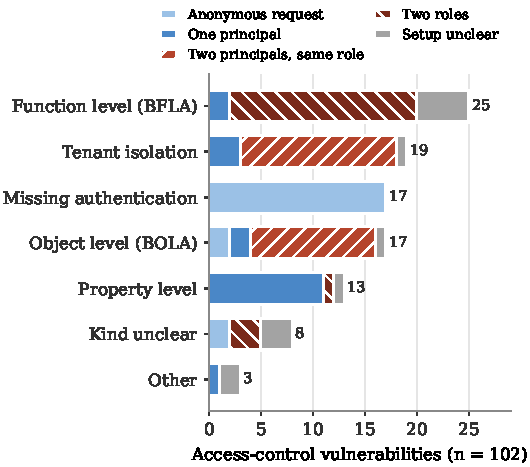
\includegraphics[width=\linewidth]{fig_r4_setup.pdf}
\caption{Minimal black-box setup that exposes each access-control vulnerability, by kind (GPT final codes, n = 102).}
\label{fig:kind}
\end{figure}

\textbf{H-R4-1 fails.} Of the 89 vulnerabilities with a decided setup, 49 need two principals (55\%; CI 45--65\%; p = 0.20). By the Claude codes the share is exactly half (40/80).

The setup follows the kind closely:
\begin{itemize}
\item all 17 missing-authentication flaws yield to an anonymous request;
\item 11 of 13 property-level flaws yield to a single principal;
\item object-level flaws need two principals of the same role (12/17);
\item tenant-isolation flaws need two principals of the same role (15/19);
\item function-level flaws need two roles (18/25).
\end{itemize}

101 of the 102 violations are observable in HTTP responses. The obstacle is therefore not observability. It is setting up the right principals and knowing what each of them may do.

\subsection{RQ3: what the contract says}
\textbf{Is the vulnerable operation described?}
\begin{itemize}
\item present: 41 (40\%);
\item absent: 29;
\item unclear: 27;
\item no usable contract: 5.
\end{itemize}

\textbf{Security requirements.} Of the 41 described operations, the contract declared a security requirement for 10. It declared none for 8, and 23 were unclear.

\textbf{H-R4-3 passes.} Consider the cases where the operation was described and the judgement was decided. In 33 of 38 of them (87\%; CI 73--94\%; p = $2.1 \times 10^{-6}$; Claude 35/39), the contract did not state the violated rule. Such a rule would be an ownership statement, a required role or scope, or a read-only property. Across all 102 vulnerabilities, the rule was stated in only 5.

\subsection{RQ4: fixes}
\textbf{H-R4-2 passes.} 93 of 102 fixes (91\%; CI 84--95\%; p = $5.0 \times 10^{-19}$) change neither a contract document nor a contract annotation. A consumer of the contract learns nothing of the fix.

\textbf{Where the fixes are made:}
\begin{itemize}
\item service logic: 30;
\item middleware or filter: 27;
\item handlers: 25;
\item model binding: 4;
\item data queries: 3;
\item other: 5;
\item unclear: 8.
\end{itemize}

Missing authentication is mostly fixed in middleware (11/17). Most property-level flaws (9/13) are fixed in service logic or model binding. 70 fixes (69\%) add or modify a test.

\subsection{Illustrative cases}
These three items are ones on which both model families agree on kind and setup.
\begin{itemize}
\item \textbf{Property-level, one principal (a Go self-hosted virtual-browser server).}
\begin{itemize}
\item \textbf{Flaw:} a profile-update operation bound the whole request body to the caller's profile, including its admin flag. Any authenticated user could make themselves administrator.
\item \textbf{Fix:} non-admins may now update only their name.
\item \textbf{Contract:} it declares a security scheme, but says nothing about which profile fields a member may set. The fix is silent.
\end{itemize}
\item \textbf{Object-level, two principals of the same role (a Mattermost Boards plugin, Go).}
\begin{itemize}
\item \textbf{Flaw:} block-modification operations did not check whether a comment belonged to the caller. Any board member could edit or delete others' comments.
\item \textbf{Fix:} a permission check is now required when the comment's creator differs from the caller.
\item \textbf{Contract:} it declares security, but not the ownership rule.
\end{itemize}
\item \textbf{Function-level, two roles (Microcks, Java).}
\begin{itemize}
\item \textbf{Flaw:} the import and export operations were reachable by non-administrators.
\item \textbf{Fix:} the role rules in the security configuration were rewritten.
\item \textbf{Contract:} this is one of the rare cases where both model families judged that the contract states the rule (administrator only). A two-role oracle could therefore check it directly.
\end{itemize}
\end{itemize}

\section{Discussion}
\begin{itemize}
\item \textbf{About half of real access-control flaws need a multi-principal setup.}
\begin{itemize}
\item Of the 89 decided cases, 40 can in principle be provoked with no principal or one principal: missing authentication, and most property-level flaws.
\item The other 49 need a deliberate multi-principal setup: two users who own different objects, or users of different roles or tenants.
\item \inferred{} This is an inference: a single-credential test configuration cannot satisfy the coded setup of those 49. We did not measure whether existing tools detect the other 40.
\item Arcuri et al.'s oracles already assume two logins~\cite{arcuri2025access}. Our data suggest that tenant boundaries and role pairs must be configured too.
\end{itemize}
\item \textbf{The contract is the wrong place to look for the policy.}
\begin{itemize}
\item Even when the vulnerable operation is documented, its contract almost never states who may do what.
\item Declared security schemes say \emph{that} credentials are needed, not \emph{whose} objects are reachable.
\item Contract-driven oracles must therefore infer the policy, for example from cross-user response comparisons or from consistency across operations~\cite{arcuri2025access}.
\item Contract authors could close part of the gap by documenting roles, scopes, ownership and read-only properties.
\end{itemize}
\item \textbf{Security fixes are silent to contract consumers.}
\begin{itemize}
\item 91\% of fixes leave the contract unchanged. This is consistent with the companion study's finding for behavioural changes, where 91\% of client-breaking silent changes touched no contract annotation.
\item Clients and gateways that rely on the contract cannot tell that an operation's access rules changed.
\end{itemize}
\item \textbf{A seed for benchmarks.}
\begin{itemize}
\item Our frozen sample has 138 advisories, each with its fix commit, the contract at the vulnerable version, and codes from two model families. It can seed a real-vulnerability benchmark.
\item Executable reproduction is future work.
\end{itemize}
\end{itemize}

\section{Threats to Validity}
\begin{itemize}
\item \textbf{Construct.}
\begin{itemize}
\item Coders judged from the advisory, the fix and the contract, without executing exploits.
\item The advisory text often describes the attack, so the setup judgement partly reflects the advisory.
\end{itemize}
\item \textbf{Contract context.}
\begin{itemize}
\item Documents were truncated to 3,000 lines. This likely explains many unclear operation judgements.
\item An over-broad attribution redaction removed 4 of the 138 advisory descriptions entirely, leaving only the summary. It removed parts of 71 more.
\end{itemize}
\item \textbf{LLM coders.}
\begin{itemize}
\item All coders are LLMs.
\item The GPT coders took 12--25 minutes for 138 items, and the Claude batches 1--3 minutes for 10--16 items. They may have relied mainly on the advisory and the diff.
\item Within-family $\kappa$ for the contract-rule judgement is only 0.62 and 0.70.
\item A human spot-check of 20 items is prepared and will be reported separately.
\end{itemize}
\item \textbf{Sampling.}
\begin{itemize}
\item Only reviewed GitHub advisories in two ecosystems with a resolvable fix commit are included, and Go dominates.
\item 831 fixes were excluded because no contract matching our detection rule existed at the vulnerable version, so contract-first projects are over-represented.
\end{itemize}
\item \textbf{Process.}
\begin{itemize}
\item The mining pipeline was implemented twice, independently by two agents.
\item After a one-line query fix to the second implementation, the two agree exactly on pool membership, SHAs, mechanical fields and sample.
\item They differ only in when the language field is computed, and in how one advisory is counted among the exclusions.
\item Four mechanical fixes were made before any coder saw a package.
\item One GPT coder was resumed after a capacity error.
\end{itemize}
\end{itemize}

\section{Conclusion}
We studied 102 real access-control vulnerabilities in OpenAPI-described REST services:
\begin{itemize}
\item Of the 89 with a decided setup, 40 can be exposed with no principal or one principal, and 49 need two users or two roles.
\item Almost all are observable over HTTP.
\item The contract rarely documents the vulnerable operation, and almost never the violated rule.
\item Fixes leave the contract unchanged.
\end{itemize}

Black-box testers need multi-principal configurations and policy inference, not only a better use of the contract.

\section*{Data availability}
An anonymised replication archive accompanies this submission ([anonymous link to be added]). It contains:
\begin{itemize}
\item the frozen plan, the scorer and the coder task;
\item both independent mining implementations, with the frozen pool and sample;
\item the key;
\item all blind packages, each with the upstream licence of every excerpt;
\item all codes;
\item a script that verifies the freezes and re-scores every coding result byte for byte.
\end{itemize}

\section*{Disclosure of AI use}
\begin{itemize}
\item \textbf{LLMs as instruments.} The study uses LLMs as measurement instruments. The GPT-family coders were \texttt{gpt-6.1-sol} via the Codex CLI, at high reasoning effort. The Claude-family coders were Claude Sonnet subagents with fresh context.
\item \textbf{LLM assistants.} The authors also used LLM assistants (Claude and Codex) to:
\begin{itemize}
\item implement and review the mining pipeline;
\item check numbers;
\item draft text.
\end{itemize}
\item \textbf{Author responsibility.} The authors reviewed all generated content and take responsibility for it.
\end{itemize}

\bibliographystyle{IEEEtran}
\bibliography{references}
\end{document}
